%=============================================================================
%  Chapter 10: Vehicle Routing Problems with Profits (VRPPs)
%  Source: Archetti, Speranza, Vigo (2014)
%  Beamer slides – self-contained lecture notes style
%=============================================================================
\documentclass[aspectratio=169,10pt]{beamer}

\usetheme{Madrid}
\usecolortheme{seahorse}

\usepackage{amsmath,amssymb,bm}
\usepackage{graphicx}
\usepackage{booktabs}
\usepackage{array}
\usepackage{xcolor}
\usepackage{listings}
\usepackage{microtype}
\usepackage{hyperref}
\usepackage{multirow}
\usepackage{tikz}

\graphicspath{{figures/}}

\lstset{
  language=Python,
  basicstyle=\ttfamily\scriptsize,
  numbers=left,
  numberstyle=\tiny\color{gray},
  frame=single,
  backgroundcolor=\color{gray!7},
  commentstyle=\color{green!50!black}\itshape,
  keywordstyle=\color{blue!80!black}\bfseries,
  stringstyle=\color{orange!80!black},
  breaklines=true,
  showstringspaces=false,
  tabsize=4,
}

\setbeamertemplate{footline}[frame number]
\setbeamertemplate{navigation symbols}{}

% ── title page ────────────────────────────────────────────────────────────────
\title[Ch.\,10: VRP with Profits]{Chapter 10: Vehicle Routing Problems with Profits}
\subtitle{Vehicle Routing: Problems, Methods, and Applications (2nd ed., 2014)}
\author{Archetti, Speranza \& Vigo}
\institute{Lecture notes prepared for self-study}
\date{2024}

%=============================================================================
\begin{document}
%=============================================================================

\begin{frame}
  \titlepage
\end{frame}

% ── table of contents ─────────────────────────────────────────────────────────
\begin{frame}[allowframebreaks]{Outline}
  \tableofcontents
\end{frame}

%=============================================================================
\section{Introduction}
%=============================================================================

\begin{frame}[allowframebreaks]{What Makes VRPPs Different?}

  In classical Vehicle Routing Problems (VRPs), the set of customers to serve
  is \emph{given in advance} and every customer must be visited.
  The Vehicle Routing Problems with Profits (VRPPs) relax this assumption
  in a fundamental way: \textbf{visiting a customer is optional}.

  \medskip
  Each customer $i$ carries a \textbf{profit} $p_i$ --- a numerical value that
  reflects how attractive it is to visit that customer.
  This profit could represent revenue collected, points scored, or any
  benefit obtained from the visit.

  \medskip
  Because customers need not all be served, the planner must make two
  intertwined decisions simultaneously:
  \begin{enumerate}
    \item \textbf{Selection:} which customers to include in the routes, and
    \item \textbf{Sequencing:} in what order to visit the chosen customers.
  \end{enumerate}

  \medskip
  A route (or a set of routes) starts and ends at a \emph{depot} and can
  be measured both in terms of \textbf{cost} (distance, time, fuel) and in
  terms of \textbf{profit} collected.
  The defining characteristic of VRPPs is that the difference between
  profit and cost can be maximised, or one of the two can be optimised
  while the other is kept within a bound.

  \framebreak

  \begin{alertblock}{Three ways to combine profit and cost}
    \begin{enumerate}
      \item \textbf{Maximise profit} subject to a \emph{cost bound} (e.g.\ a
            time limit $T_{\max}$): collect as much profit as possible
            without exceeding the budget.
      \item \textbf{Minimise cost} subject to a \emph{profit threshold}
            $P_{\min}$: travel as little as possible while still collecting
            at least $P_{\min}$ profit.
      \item \textbf{Maximise (profit $-$ cost)}: find the route for which
            the net benefit is greatest, with no hard constraints on either.
    \end{enumerate}
  \end{alertblock}

\end{frame}

\begin{frame}[allowframebreaks]{Real-World Applications}

  VRPPs arise in many practical settings.
  In each case the key idea is that it is not always worth visiting every
  location --- visiting a low-profit customer far from the depot may cost
  more than the benefit gained.

  \medskip
  \begin{itemize}
    \item \textbf{Steel rolling mill scheduling.} A rolling mill
          can produce items for some customers during a given shift.
          Not all orders can be fulfilled; the scheduler selects which
          orders to accept to maximise throughput.
          (Balas, 1989; 1993)

    \item \textbf{Tourist trip design.} Given a fixed vacation time,
          a tourist visits a subset of attractions.
          Each attraction has a ``score'' (profit).
          The goal is to plan the itinerary that maximises total score
          within the time budget.
          (Vansteenwegen \& Van~Oudheusden, 2007)

    \item \textbf{Auditor routing.} A limited number of auditors must visit
          suppliers.
          The profit is the amount of recovered claims.
          Not all suppliers can be audited; the scheduler selects the most
          profitable ones.
          (Ilhan, Iravani \& Daskin, 2008)

    \item \textbf{Sports recruiting.} A college recruiter has limited travel
          days to visit high schools and recruit athletes.
          Each school has an estimated recruitment value (profit).
          (Butt \& Cavalier, 1994)

    \item \textbf{Salesperson planning.} A salesperson cannot call on all
          clients each week; she selects those offering the highest expected
          commission.
          (Ramesh \& Brown, 1991)

    \item \textbf{Oil tanker routing.} An oil company routes tankers to
          serve ships at sea.
          Demand at each location is known; only a subset of ships can be
          refuelled per voyage.
          (Golden, Levy \& Vohra, 1987)

    \item \textbf{Home-care delivery.} A company delivers home-care products.
          Not all customers need delivery every day; a maximum distance is
          imposed on each route.
          (Savelsbergh \& Sol, 1995)

    \item \textbf{Unmanned aerial vehicle (UAV) mission planning.}
          A UAV has limited battery.
          It visits a subset of targets to collect information, maximising
          total intelligence value collected.
  \end{itemize}

\end{frame}

\begin{frame}[allowframebreaks]{The VRPP Family: Taxonomy}

  \begin{figure}
    \centering
    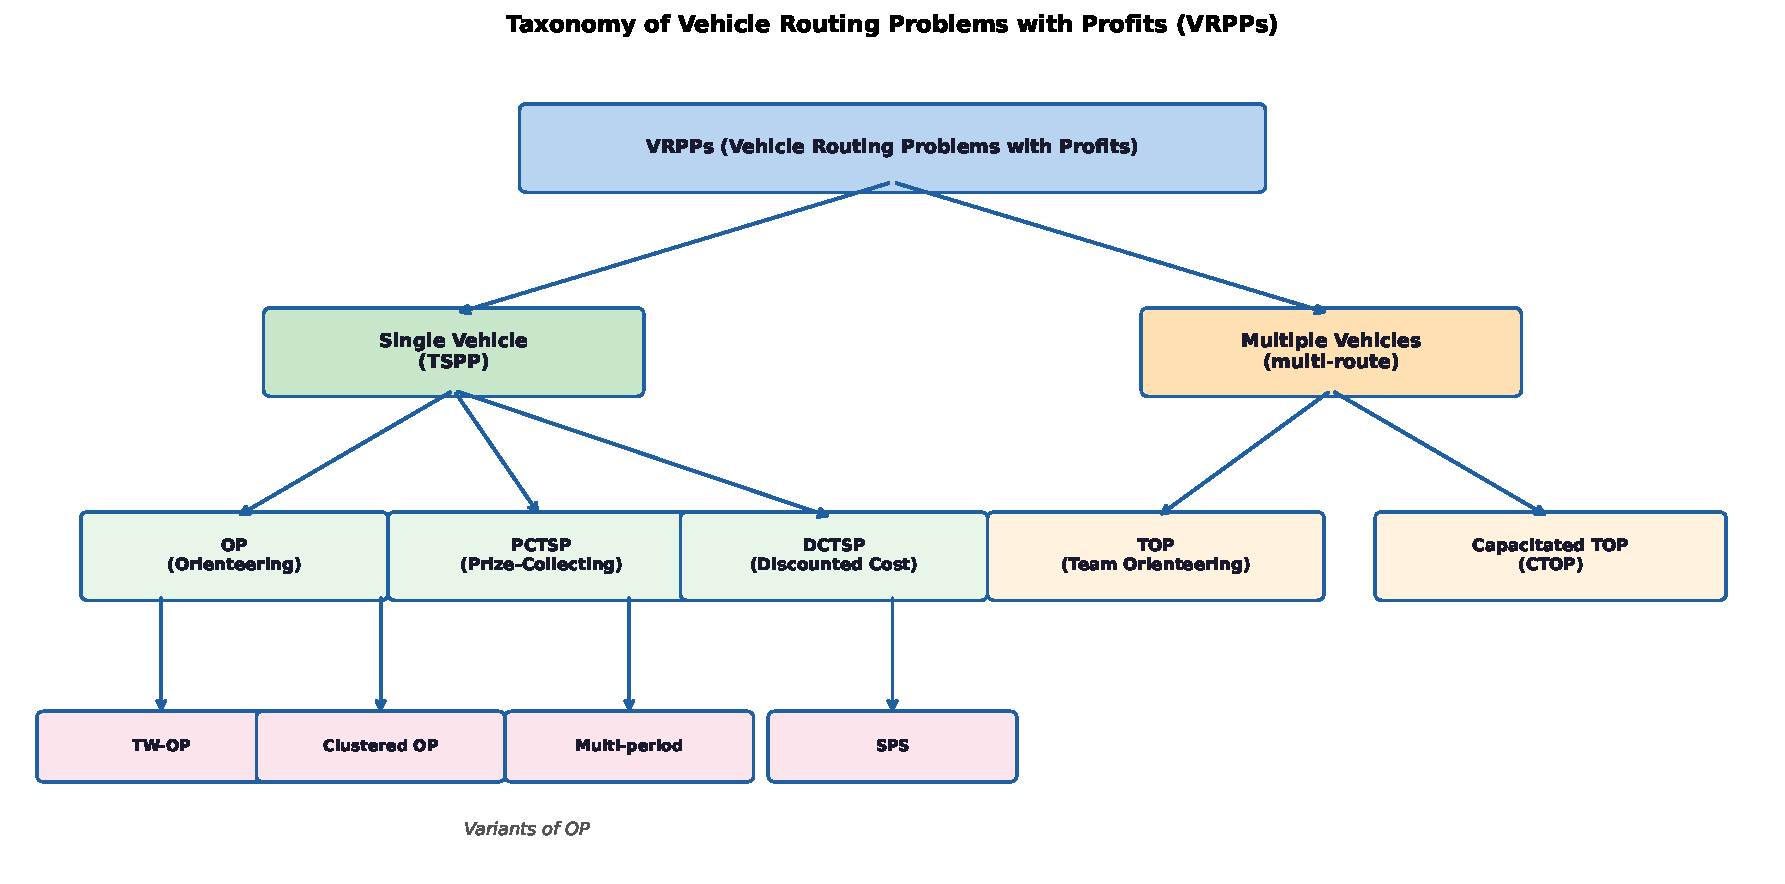
\includegraphics[width=0.90\linewidth]{fig_taxonomy.pdf}
    \caption{Taxonomy of Vehicle Routing Problems with Profits.
             Single-vehicle variants form the \emph{Travelling Salesman
             Problem with Profits (TSPP)} family.
             Multi-vehicle variants form the \emph{Team Orienteering Problem
             (TOP)} family.}
  \end{figure}

  \medskip
  The taxonomy splits naturally along two dimensions:
  (1) single vehicle vs.\ multiple vehicles, and
  (2) the type of objective (maximise profit, minimise cost, or maximise
  net profit).
  Many real-world extensions add further structure: time windows,
  clustered customers, multi-period planning, or stochastic profits.

\end{frame}

\begin{frame}[allowframebreaks]{Summary Table of VRPP Variants}

  The following table summarises the main problem classes studied in this
  chapter.
  Column \emph{Objective} shows what is optimised;
  column \emph{Constraint} shows the binding restriction that makes the
  problem non-trivial.

  \medskip
  \begin{center}
  \small
  \begin{tabular}{lllc}
    \toprule
    \textbf{Problem} & \textbf{Objective} & \textbf{Key Constraint} & \textbf{Vehicles} \\
    \midrule
    OP  (Orienteering)           & Max profit       & Travel time $\le T_{\max}$  & 1  \\
    PCTSP (Prize-Collecting TSP) & Min cost $+$ penalties & Min profit $\ge P_{\min}$ & 1  \\
    DCTSP (Discounted-Cost TSP)  & Max profit $-$ cost  & None                    & 1  \\
    TOP  (Team Orienteering)     & Max total profit & Each route $\le T_{\max}$   & $m$  \\
    CTOP (Capacitated TOP)       & Max total profit & Demand $\le Q$ per route    & $m$  \\
    TW-OP / TW-TOP               & Max profit       & Time windows $[a_i, b_i]$   & 1/$m$ \\
    Clustered OP                 & Max profit       & Visit whole cluster or none & 1  \\
    Multi-period TOP             & Max total profit & Period planning horizon      & $m$  \\
    \bottomrule
  \end{tabular}
  \end{center}

  \medskip
  In the table, $T_{\max}$ (T-max) is the maximum allowed travel time or
  distance per route; $P_{\min}$ (P-min) is a minimum profit threshold;
  $Q$ (Q) is the vehicle capacity; $m$ is the number of vehicles;
  and $[a_i, b_i]$ (a-sub-i to b-sub-i) is the time window for customer
  $i$ --- the interval during which the vehicle must arrive.

\end{frame}

%=============================================================================
\section{Single-Vehicle Case}
%=============================================================================

\begin{frame}[allowframebreaks]{Graph Notation and Problem Setup}

  All VRPP variants are defined on a \textbf{directed graph}
  (or equivalently an undirected graph for symmetric costs).
  We define the notation once here and reuse it throughout.

  \medskip
  \begin{block}{Graph Notation}
    \begin{itemize}
      \item $G = (V, A)$: a complete directed graph where $V$ is the set of
            nodes and $A$ is the set of arcs (directed edges).
      \item $V = \{0, 1, 2, \ldots, n\}$: node $0$ is the \emph{depot}
            (starting and ending point); nodes $1, \ldots, n$ are the
            \emph{customers} (potential stops).
      \item $p_i \ge 0$: profit associated with customer $i \in V \setminus \{0\}$.
            This is the reward collected when customer $i$ is visited.
      \item $c_{ij} \ge 0$: travel cost (distance or time) from node $i$
            to node $j$.
            In most instances, $c_{ij}$ is the Euclidean distance between
            two points in the plane.
      \item $x_{ij} \in \{0, 1\}$: binary decision variable.
            $x_{ij} = 1$ if the vehicle travels directly from node $i$ to
            node $j$; otherwise $x_{ij} = 0$.
      \item $y_i \in \{0, 1\}$: binary decision variable.
            $y_i = 1$ if customer $i$ is visited; otherwise $y_i = 0$.
    \end{itemize}
  \end{block}

  \medskip
  The subscript notation $x_{ij}$ is read ``x sub i j''.
  Think of $x_{ij}$ as a switch: it is 1 (on) if the route uses the road
  segment from $i$ to $j$, and 0 (off) otherwise.

\end{frame}

%=============================================================================
\subsection{Orienteering Problem (OP)}
%=============================================================================

\begin{frame}[allowframebreaks]{The Orienteering Problem (OP): Intuition}

  The Orienteering Problem (OP) takes its name from the outdoor sport of
  orienteering, where competitors collect checkpoints within a fixed time.
  The mathematical problem asks the same question:
  \textbf{which checkpoints (customers) can I visit within a given time limit,
  and in what order, so as to collect the most points (profit)?}

  \medskip
  The OP was first introduced by Tsiligirides (1984) and later formally
  defined by Golden, Levy, and Vohra (1987).
  It is a single-vehicle problem: one vehicle (or person) starts at the
  depot, visits a subset of customers, and returns to the depot, all within
  a maximum travel time $T_{\max}$ (T-max).

  \begin{figure}
    \centering
    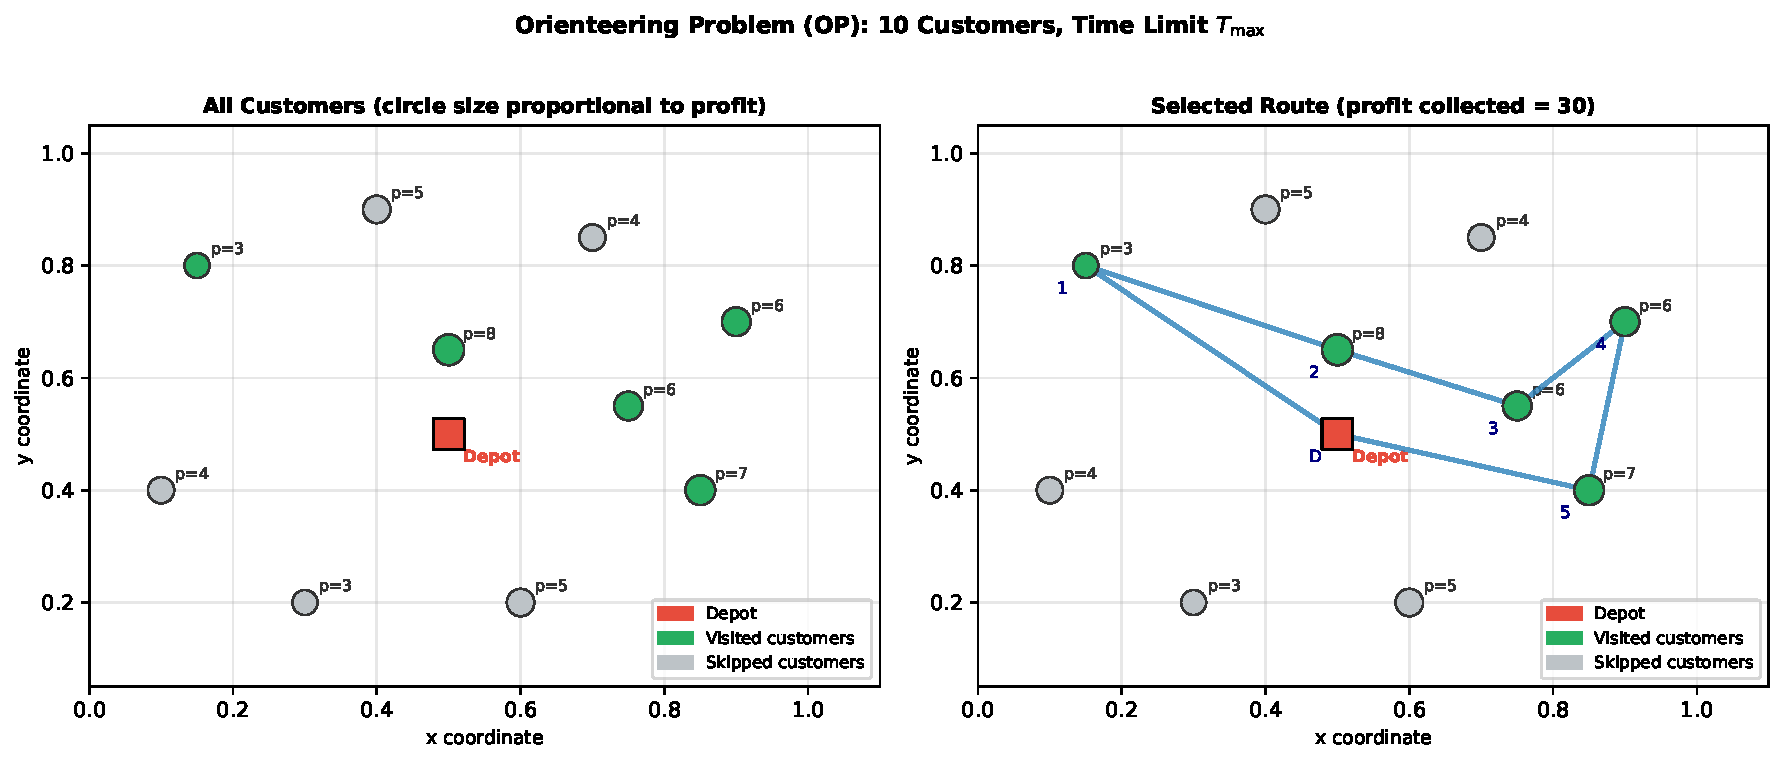
\includegraphics[width=0.60\linewidth]{fig_op_example.pdf}
    \caption{Left: all 10 customers, circle size proportional to profit.
             Right: the selected route (blue path) visits 5 customers and
             collects profit equal to their sum.
             The remaining customers are skipped because including them would
             violate the time limit.}
  \end{figure}

\end{frame}

\begin{frame}[allowframebreaks]{OP Mathematical Formulation}

  We now state the OP as an integer program.
  Every constraint is explained in full.

  \medskip
  \begin{block}{Orienteering Problem (OP) -- Integer Program}
    \textbf{Maximise}
    \[
      \sum_{i \in V} p_i \, y_i
      \tag{OP.obj}
    \]
    \textbf{Subject to}
    \begin{align}
      \sum_{j \in V} x_{0j} &= 1
      \tag{OP.1} \\
      \sum_{j \in V} x_{j0} &= 1
      \tag{OP.2} \\
      \sum_{j \in V} x_{ij} &= y_i
      \quad \forall\, i \in V \setminus \{0\}
      \tag{OP.3} \\
      \sum_{j \in V} x_{ji} &= y_i
      \quad \forall\, i \in V \setminus \{0\}
      \tag{OP.4} \\
      \sum_{(i,j) \in A} c_{ij} \, x_{ij} &\le T_{\max}
      \tag{OP.5} \\
      x_{ij} &\in \{0,1\}
      \quad \forall\, (i,j) \in A
      \tag{OP.6} \\
      y_i    &\in \{0,1\}
      \quad \forall\, i \in V
      \tag{OP.7}
    \end{align}
  \end{block}

  \framebreak

  \begin{block}{Explanation of Each Constraint}
    \begin{itemize}
      \item \textbf{(OP.obj)} The objective function says: maximise the
            total profit collected from all visited customers.
            Here $p_i$ (p sub i) is the profit of customer $i$, and
            $y_i$ (y sub i) equals 1 if customer $i$ is visited, 0 otherwise.
            The symbol $\Sigma$ (Sigma, meaning ``sum'') runs over all
            nodes $i$ in the set $V$.

      \item \textbf{(OP.1)} Exactly one arc leaves the depot (node 0).
            This means the route starts with a single trip away from home.

      \item \textbf{(OP.2)} Exactly one arc enters the depot.
            The route must return to home exactly once.

      \item \textbf{(OP.3)} If customer $i$ is visited ($y_i = 1$), then
            exactly one arc leaves node $i$ (the vehicle departs).
            If customer $i$ is not visited ($y_i = 0$), no arc leaves it.

      \item \textbf{(OP.4)} Symmetric to (OP.3) for arcs entering $i$.
            Together (OP.3) and (OP.4) enforce \emph{flow conservation}:
            every visited customer has one arrival and one departure.

      \item \textbf{(OP.5)} The total travel cost of all arcs used must not
            exceed $T_{\max}$ (T-max), the time or distance budget.
            This is the ``time limit'' constraint that prevents visiting
            all customers.

      \item \textbf{(OP.6, OP.7)} Integrality: all decision variables are
            binary (0 or 1).
    \end{itemize}
  \end{block}

  \medskip
  \begin{alertblock}{Key Insight: What the OP Balances}
    The OP balances two forces.
    Including more customers increases the objective (more profit) but also
    increases the total travel time, which can violate constraint (OP.5).
    The optimal solution visits exactly those customers for which the
    profit gain justifies the extra travel cost within the budget.
    Customers far from the route or with low profit are skipped.
  \end{alertblock}

  \framebreak

  Note: constraints (OP.1)--(OP.4) do not prevent \emph{subtours}
  (disconnected loops that do not pass through the depot).
  To prevent subtours, additional constraints are needed.
  Two standard approaches are:
  \begin{enumerate}
    \item \textbf{Miller-Tucker-Zemlin (MTZ) constraints:}
          introduce a continuous variable $u_i$ (u sub i, representing the
          position of customer $i$ in the route) and add
          $u_i - u_j + n \cdot x_{ij} \le n - 1$ for all $i \neq j$.
    \item \textbf{Subtour elimination constraints:}
          for every subset $S \subseteq V \setminus \{0\}$,
          require $\sum_{(i,j): i \in S, j \in S} x_{ij} \le |S| - 1$.
          There are exponentially many such constraints, so they are
          added lazily in a branch-and-cut algorithm.
  \end{enumerate}

\end{frame}

\begin{frame}[allowframebreaks]{OP: A Worked Numerical Example}

  We illustrate the OP with 5 customers and a small time limit.
  Customers are located in the plane; the depot is at the origin $(0,0)$.

  \medskip
  \begin{exampleblock}{Instance}
    \begin{center}
    \begin{tabular}{cccc}
      \toprule
      Customer & $x$ & $y$ & Profit $p_i$ \\
      \midrule
      Depot (0) & 0 & 0 & -- \\
      1 & 1 & 2 & 5 \\
      2 & 3 & 1 & 8 \\
      3 & 4 & 3 & 6 \\
      4 & 2 & 4 & 4 \\
      5 & 5 & 2 & 9 \\
      \bottomrule
    \end{tabular}
    \end{center}
    Time limit: $T_{\max} = 12$.
    Travel cost $c_{ij}$ is Euclidean distance (rounded to 1 decimal place).
  \end{exampleblock}

  \medskip
  \textbf{Relevant distances:}
  \begin{itemize}
    \item $c_{01} = \sqrt{1^2+2^2} \approx 2.2$,\quad
          $c_{02} = \sqrt{3^2+1^2} \approx 3.2$,\quad
          $c_{05} = \sqrt{5^2+2^2} \approx 5.4$
    \item $c_{12} = \sqrt{(3-1)^2+(1-2)^2} \approx 2.2$,\quad
          $c_{25} = \sqrt{(5-3)^2+(2-1)^2} \approx 2.2$,\quad
          $c_{50} = 5.4$
  \end{itemize}

  \medskip
  \textbf{Route Candidate A:} Depot $\to$ 1 $\to$ 2 $\to$ 5 $\to$ Depot.\\
  Cost $= 2.2 + 2.2 + 2.2 + 5.4 = 12.0 \le T_{\max}$. Profit $= 5+8+9 = 22$.

  \medskip
  \textbf{Route Candidate B:} Depot $\to$ 2 $\to$ 3 $\to$ 5 $\to$ Depot.\\
  Cost $= 3.2 + \sqrt{(4-3)^2+(3-1)^2} + \sqrt{(5-4)^2+(2-3)^2} + 5.4
        \approx 3.2 + 2.2 + 1.4 + 5.4 = 12.2 > T_{\max}$. \textbf{Infeasible.}

  \medskip
  \textbf{Conclusion:} Route A is feasible and collects profit 22.
  Adding customer 3 or 4 pushes cost above 12.
  Route A is optimal for this instance.

  \begin{alertblock}{Key Insight}
    With only 5 customers, checking all $2^5=32$ subsets is feasible
    by hand. For $n=100$ customers, brute force requires checking $2^{100}$
    subsets --- impossible without intelligent algorithms.
    This is why the OP is NP-hard and requires sophisticated methods.
  \end{alertblock}

\end{frame}

\begin{frame}[allowframebreaks]{OP: Exact Algorithms}

  The OP is NP-hard (non-deterministic polynomial time hard), meaning no
  known algorithm solves it optimally in time that grows polynomially
  with $n$ (the number of customers).
  Despite this, exact algorithms can solve instances of moderate size.

  \medskip
  \textbf{Branch and Bound (B\&B).}
  Tsiligirides (1984) first proposed the OP and solved it using B\&B.
  The algorithm builds a tree of partial solutions.
  At each node it computes an \emph{upper bound} on the best possible
  profit achievable from that partial solution.
  If the upper bound is less than the best complete solution found so far,
  the branch is pruned (discarded).
  Laporte and Martello (1990) developed stronger upper bounds
  based on a relaxation of the time constraint, reducing the tree size.

  \medskip
  \textbf{Dynamic Programming (DP).}
  Tsiligirides (1984) also proposed a DP approach.
  The state is the set of customers already visited and the current
  node; the value function stores the maximum profit achievable.
  DP is exact but requires memory exponential in $n$ (the state space
  grows as $2^n \times n$), so it is practical only for $n \lesssim 20$.

  \medskip
  \textbf{Branch and Cut (B\&C).}
  Fischetti, Salazar-Gonz\'alez, and Toth (1998) developed a
  branch-and-cut approach using subtour elimination constraints added
  dynamically.
  This method can solve instances with up to about 100 customers
  to optimality.

  \medskip
  \textbf{Integer Linear Programming (ILP) / Branch and Price.}
  For larger instances, column generation combined with B\&B
  (branch-and-price) has been used.
  Each column in the master problem corresponds to a complete route;
  the pricing subproblem finds the most profitable route to add.

\end{frame}

\begin{frame}[allowframebreaks]{OP: Approximation Results}

  Because the OP is NP-hard, researchers have studied how well
  polynomial-time algorithms can approximate the optimal solution.

  \medskip
  \begin{block}{Approximation Hardness}
    The OP cannot be approximated within any constant factor in polynomial
    time unless P = NP (where P and NP are complexity classes).
    Intuitively, this is because the subset-selection and routing decisions
    are tightly coupled.
  \end{block}

  \medskip
  Blum et al.\ (2003) proposed the first polynomial-time approximation
  scheme (PTAS) for a special case where the time limit is large enough
  to visit most customers.
  Chekuri et al.\ (2012) showed that the OP can be approximated within a
  factor of $(1 + 1/\varepsilon)$ (1 plus 1-over-epsilon) for any
  $\varepsilon > 0$ (epsilon greater than zero) when using a quasi-polynomial
  algorithm (running in time $n^{O(\log n)}$).

  \medskip
  \begin{alertblock}{Practical Implication}
    For the instances sizes arising in practice (typically $n \le 300$),
    metaheuristics (Tabu Search, Simulated Annealing, ILS) find solutions
    within 1--2\% of optimal in seconds, making them the method of choice.
  \end{alertblock}

\end{frame}

\begin{frame}[allowframebreaks]{OP: Heuristic Algorithms -- Greedy Construction}

  Greedy construction heuristics build a solution step by step, adding
  one customer at a time without backtracking.
  They are fast but may miss the global optimum.

  \medskip
  \textbf{The Profit-per-Cost Ratio Heuristic.}
  The simplest greedy approach ranks customers by their profit-to-distance
  ratio and inserts them greedily:

  \medskip
  \begin{enumerate}
    \item Compute the ratio $r_i = p_i / c_{0i}$ (r sub i = profit of
          customer $i$ divided by distance from depot to $i$) for each
          customer.
    \item Sort customers by $r_i$ in decreasing order.
    \item Starting from an empty route (depot $\to$ depot), insert the
          next customer from the sorted list into the cheapest position
          in the current route, as long as the time limit is not violated.
    \item Repeat until no more customers can be inserted without
          exceeding $T_{\max}$.
  \end{enumerate}

  \medskip
  \textbf{Worked example} (5 customers from the previous slide):
  \begin{itemize}
    \item Ratios: $r_1 = 5/2.2 \approx 2.3$,\;
                  $r_2 = 8/3.2 = 2.5$,\;
                  $r_3 = 6/5.1 \approx 1.2$,\;
                  $r_4 = 4/4.5 \approx 0.9$,\;
                  $r_5 = 9/5.4 \approx 1.7$.
    \item Sorted order: $2, 1, 5, 3, 4$.
    \item Insert customer 2: route = D $\to$ 2 $\to$ D, cost = $3.2 + 3.2 = 6.4$.
    \item Insert customer 1: route = D $\to$ 1 $\to$ 2 $\to$ D,
          cost $= 2.2 + 2.2 + 3.2 = 7.6$.
    \item Insert customer 5: route = D $\to$ 1 $\to$ 2 $\to$ 5 $\to$ D,
          cost $= 2.2 + 2.2 + 2.2 + 5.4 = 12.0 \le 12$. \checkmark
    \item Insert customer 3: would cost $> 12$. Stop.
    \item Final profit $= 5 + 8 + 9 = 22$. (Optimal for this instance.)
  \end{itemize}

\end{frame}

\begin{frame}[allowframebreaks]{OP: Heuristic Algorithms -- GRASP and ILS}

  More sophisticated heuristics combine construction with local search
  improvement.

  \medskip
  \textbf{GRASP (Greedy Randomised Adaptive Search Procedure).}
  GRASP was applied to the OP by Fischetti, Salazar-Gonz\'alez, and Toth
  (1998).
  Each iteration has two phases:
  \begin{enumerate}
    \item \textbf{Construction phase:} at each step, instead of always
          inserting the single best customer, build a \emph{Restricted
          Candidate List (RCL)} of the top $k$ candidates by profit/cost
          ratio, then select one at random from the RCL.
          This introduces controlled randomness.
    \item \textbf{Local search phase:} improve the constructed solution by
          applying 2-opt or 3-opt exchanges (removing 2 or 3 edges and
          reconnecting in a better order) and swap moves (exchanging a
          visited customer with an unvisited one if it improves profit).
  \end{enumerate}
  The best solution across all iterations is retained.
  GRASP is easy to parallelise because iterations are independent.

  \medskip
  \textbf{ILS (Iterated Local Search).}
  Vansteenwegen, Souffriau, and Van~Oudheusden (2009) developed a very
  effective ILS for the OP and TOP.
  ILS alternates between:
  \begin{itemize}
    \item a \textbf{perturbation step} that randomly removes some customers
          and re-inserts others (escaping local optima), and
    \item a \textbf{local search step} that applies 2-opt, Or-opt, and
          customer swap moves until no improvement is found.
  \end{itemize}
  ILS achieved near-optimal results on all standard OP benchmarks
  in fractions of a second.

\end{frame}

%=============================================================================
\subsection{Prize-Collecting TSP (PCTSP)}
%=============================================================================

\begin{frame}[allowframebreaks]{Prize-Collecting TSP (PCTSP)}

  The Prize-Collecting Travelling Salesman Problem (PCTSP) was introduced
  by Balas (1989) to model steel rolling mill scheduling.
  It differs from the OP in both the objective and the constraint structure.

  \medskip
  In the PCTSP:
  \begin{itemize}
    \item Each customer $i$ has a \textbf{profit} $p_i$ (reward for visiting)
          and a \textbf{penalty} $\pi_i$ (pi sub i, pronounced ``pie sub i'')
          that is paid if customer $i$ is \emph{not} visited.
    \item The objective is to \textbf{minimise total travel cost plus total
          penalties} for unvisited customers.
    \item There is a \textbf{minimum profit constraint}: the total profit
          collected must be at least $P_{\min}$ (P-min).
  \end{itemize}

  \medskip
  \begin{block}{PCTSP -- Integer Program}
    \textbf{Minimise}
    \[
      \sum_{(i,j) \in A} c_{ij} \, x_{ij}
      + \sum_{i \in V \setminus \{0\}} \pi_i (1 - y_i)
      \tag{PCTSP.obj}
    \]
    \textbf{Subject to}
    \[
      \sum_{i \in V \setminus \{0\}} p_i \, y_i \ge P_{\min}
      \tag{PCTSP.profit}
    \]
    plus the same flow conservation constraints as the OP.
  \end{block}

  \framebreak

  \begin{block}{Explanation of the PCTSP Objective}
    The objective function (PCTSP.obj) has two parts:
    \begin{enumerate}
      \item $\sum_{(i,j)} c_{ij} x_{ij}$: total travel cost for all arcs
            used.
            Here $c_{ij}$ (c sub i j) is the cost of traveling from node
            $i$ to node $j$, and $x_{ij}$ (x sub i j) is 1 if that arc is
            used.
      \item $\sum_{i} \pi_i (1 - y_i)$: total penalty for unvisited
            customers.
            Here $\pi_i$ (pi sub i) is the penalty for skipping customer
            $i$, and $(1 - y_i)$ equals 1 if customer $i$ is skipped.
    \end{enumerate}
    The minimisation balances these two costs: travelling further reduces
    penalties but increases route cost.
  \end{block}

  \medskip
  \begin{alertblock}{PCTSP vs OP}
    In the OP, the time limit is a \emph{hard constraint} and the objective
    is to maximise profit.
    In the PCTSP, the minimum profit is a \emph{hard constraint} and the
    objective is to minimise cost plus penalties.
    Both are equivalent in the limit (one can be converted to the other
    by parameterising $T_{\max}$ or $P_{\min}$), but they model different
    real-world priorities.
  \end{alertblock}

  \medskip
  \textbf{Exact algorithms for the PCTSP.}
  Fischetti and Toth (1988) introduced the first exact algorithm.
  Bienstock, Goemans, Simchi-Levi, and Williamson (1993) showed that
  the PCTSP admits a 2-approximation (a polynomial algorithm guaranteed
  to find a solution within a factor of 2 of optimal).

\end{frame}

%=============================================================================
\subsection{Profitable Tour Problem (PTP / DCTSP)}
%=============================================================================

\begin{frame}[allowframebreaks]{Profitable Tour Problem (PTP) and DCTSP}

  The Profitable Tour Problem (PTP), also called the Discounted-Cost TSP
  (DCTSP), takes yet another approach to balancing profit and cost.

  \medskip
  In the PTP:
  \begin{itemize}
    \item There is \textbf{no hard constraint} on either total travel cost
          or minimum profit.
    \item Each customer $i$ has a profit $p_i$ for visiting and a cost
          $c_{ij}$ for each arc.
    \item The objective is to \textbf{maximise net profit}:
          total collected profit minus total travel cost.
  \end{itemize}

  \medskip
  \begin{block}{PTP -- Objective}
    \textbf{Maximise}
    \[
      \sum_{i \in V \setminus \{0\}} p_i \, y_i
      - \sum_{(i,j) \in A} c_{ij} \, x_{ij}
      \tag{PTP.obj}
    \]
    Subject to the same flow conservation and integrality constraints as
    the OP (but without the time limit constraint OP.5).
  \end{block}

  \medskip
  Here $\sum_{i} p_i y_i$ (Sigma p sub i y sub i) is the total profit
  from visited customers, and $\sum_{(i,j)} c_{ij} x_{ij}$
  (Sigma c sub i j times x sub i j) is the total travel cost.
  The difference is maximised.

  \medskip
  \textbf{Key behavioural observation.}
  In the PTP, a customer $i$ is worth visiting only if its profit $p_i$
  exceeds the detour cost of including it.
  Formally, customer $i$ is worth adding to a route that currently goes
  from node $a$ to node $b$ if
  $p_i > c_{ai} + c_{ib} - c_{ab}$
  (the profit exceeds the savings lost from the detour).

  \medskip
  \textbf{Exact algorithms.}
  Del Pia and Filippi (2006) and Archetti, Hertz, and Speranza (2007)
  studied exact and heuristic methods.
  Archetti et al.\ proposed a branch-and-cut approach that adds subtour
  elimination and optimality cuts dynamically.

\end{frame}

%=============================================================================
\section{Multiple-Vehicle Case}
%=============================================================================

\begin{frame}[allowframebreaks]{From Single to Multiple Vehicles}

  When a single vehicle cannot collect enough profit within the time limit,
  deploying a \textbf{fleet of vehicles} becomes necessary.
  Multiple vehicles depart from the same depot, each follows an
  independent route within the time limit $T_{\max}$, and together
  they aim to collect the maximum total profit.

  \medskip
  The transition from the OP to the Team Orienteering Problem (TOP)
  is analogous to the transition from the TSP to the VRP:
  we add more vehicles and ask how to partition the customers among them
  optimally.

  \medskip
  \begin{block}{New notation for multi-vehicle problems}
    \begin{itemize}
      \item $m$: number of vehicles in the fleet.
      \item $k \in \{1, \ldots, m\}$: index for vehicles.
      \item $x_{ijk} \in \{0,1\}$: equals 1 if vehicle $k$ travels
            directly from node $i$ to node $j$.
      \item $y_{ik} \in \{0,1\}$: equals 1 if vehicle $k$ visits
            customer $i$.
      \item $T_{\max}$: maximum travel time (or distance) allowed
            for each individual vehicle's route.
    \end{itemize}
  \end{block}

  \medskip
  A customer can be visited by \textbf{at most one vehicle}.
  If customer $i$ is visited, exactly one vehicle serves it.
  This prevents double-counting profits.

\end{frame}

%=============================================================================
\subsection{Team Orienteering Problem (TOP)}
%=============================================================================

\begin{frame}[allowframebreaks]{Team Orienteering Problem (TOP): Definition}

  The Team Orienteering Problem (TOP) was introduced by
  Chao, Golden, and Wasil (1996).
  It generalises the OP to $m$ vehicles:
  \textbf{find $m$ routes, each starting and ending at the depot and not
  exceeding $T_{\max}$, so that the total collected profit is maximised}.

  \begin{figure}
    \centering
    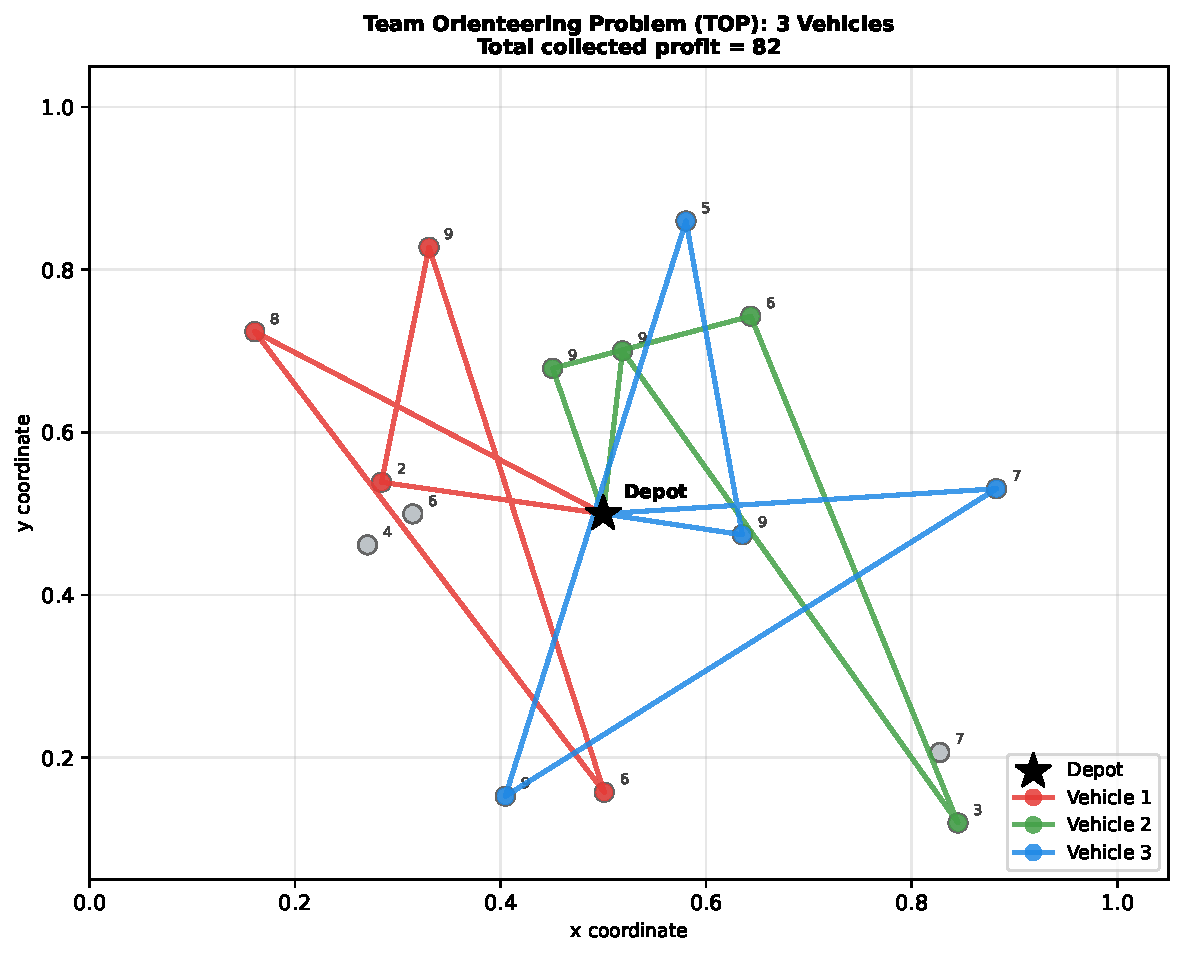
\includegraphics[width=0.60\linewidth]{fig_top_example.pdf}
    \caption{TOP with 3 vehicles and 15 customers.
             Each coloured path is one vehicle's route.
             Not all customers are visited; the selection maximises
             total profit within the time limit.}
  \end{figure}

\end{frame}

\begin{frame}[allowframebreaks]{TOP: Mathematical Formulation}

  We present the full integer programming formulation for the directed TOP.

  \medskip
  \begin{block}{Team Orienteering Problem -- Integer Program}
    \textbf{Maximise}
    \[
      \sum_{k=1}^{m} \sum_{i \in V} p_i \, y_{ik}
      \tag{TOP.obj}
    \]
    \textbf{Subject to}
    \begin{align}
      \sum_{k=1}^{m} \sum_{j \in V} x_{0jk} &= m
      \tag{TOP.1}\\
      \sum_{j \in V} x_{0jk} &= 1
      \quad \forall\, k
      \tag{TOP.2}\\
      \sum_{j \in V} x_{j0k} &= 1
      \quad \forall\, k
      \tag{TOP.3}\\
      \sum_{j \in V} x_{ijk} &= y_{ik}
      \quad \forall\, i \in V \setminus\{0\},\, k
      \tag{TOP.4}\\
      \sum_{j \in V} x_{jik} &= y_{ik}
      \quad \forall\, i \in V \setminus\{0\},\, k
      \tag{TOP.5}\\
      \sum_{k=1}^{m} y_{ik} &\le 1
      \quad \forall\, i \in V \setminus\{0\}
      \tag{TOP.6}\\
      \sum_{(i,j) \in A} c_{ij} \, x_{ijk} &\le T_{\max}
      \quad \forall\, k
      \tag{TOP.7}\\
      x_{ijk} &\in \{0,1\},\quad y_{ik} \in \{0,1\}
      \tag{TOP.8}
    \end{align}
  \end{block}

  \framebreak

  \begin{block}{Constraint Explanations}
    \begin{itemize}
      \item \textbf{(TOP.obj)} Maximise the sum of profits over all vehicles
            $k$ and all customers $i$ that vehicle $k$ visits.
            $y_{ik}$ (y sub i k) equals 1 if vehicle $k$ visits customer $i$.

      \item \textbf{(TOP.1)} All $m$ vehicles leave the depot.
            The total number of departure arcs from node 0 equals $m$.

      \item \textbf{(TOP.2)} Each vehicle $k$ leaves the depot exactly once.

      \item \textbf{(TOP.3)} Each vehicle $k$ returns to the depot exactly once.

      \item \textbf{(TOP.4, TOP.5)} Flow conservation for vehicle $k$ at
            customer $i$: if vehicle $k$ visits customer $i$, then exactly
            one arc enters $i$ via vehicle $k$ and one arc leaves $i$ via
            vehicle $k$.

      \item \textbf{(TOP.6)} Each customer $i$ is visited by \emph{at most
            one} vehicle.
            This prevents double-counting the profit of customer $i$.

      \item \textbf{(TOP.7)} The total travel cost of vehicle $k$'s route
            must not exceed $T_{\max}$.
            Each vehicle has the same time budget.

      \item \textbf{(TOP.8)} All decision variables are binary.
    \end{itemize}
  \end{block}

  \begin{alertblock}{Why TOP is Harder than OP}
    The TOP is harder than the OP because we must also decide how to
    \emph{allocate} customers across vehicles.
    Even if we knew which customers to visit, partitioning them into
    $m$ time-feasible routes is itself an NP-hard bin-packing-like problem.
    The interaction between selection and allocation is what makes the TOP
    challenging.
  \end{alertblock}

\end{frame}

\begin{frame}[allowframebreaks]{TOP: Heuristic Algorithms}

  Because the TOP is NP-hard, heuristic methods dominate the practical
  literature.
  The following approaches have been most successful.

  \medskip
  \textbf{1. Greedy Algorithm (Chao, Golden, Wasil 1996).}
  The first heuristic for the TOP proceeds greedily:
  \begin{enumerate}
    \item For each vehicle $k$ in turn, select the unvisited customer with
          the best profit-per-distance ratio that can be inserted without
          violating $T_{\max}$.
    \item Insert it into the cheapest position in vehicle $k$'s current route.
    \item Repeat until no more insertions are feasible.
  \end{enumerate}
  This is fast ($O(n^2 m)$ time) but may be far from optimal because
  it does not reconsider earlier decisions.

  \medskip
  \textbf{2. Simulated Annealing (SA) (Chiang and Wang, 1996).}
  Simulated Annealing mimics the physical process of cooling a metal.
  A hot metal can move to a higher-energy state (worse solution) with
  non-zero probability; as it cools, the probability of accepting worse
  solutions decreases.
  In the TOP context:
  \begin{itemize}
    \item The ``temperature'' $T$ (T) starts high and is reduced by
          a cooling factor $\alpha$ (alpha) at each iteration:
          $T \leftarrow \alpha \cdot T$.
    \item At each step, a \emph{neighbour solution} is generated by
          swapping a visited and an unvisited customer, or by removing one
          customer and inserting another.
    \item If the neighbour is better, accept it always.
          If it is worse (profit decreases by $\Delta$ (Delta)), accept it
          with probability $e^{-\Delta / T}$ (e to the minus Delta over T).
          This is the \emph{Metropolis criterion}.
    \item As $T \to 0$ (T approaches zero), the algorithm becomes greedy
          and converges to a local optimum.
  \end{itemize}

  \framebreak

  \textbf{3. Tabu Search (TS) (Tang and Miller-Hooks, 2005).}
  Tabu Search avoids cycling by maintaining a \emph{tabu list} --- a memory
  of recently made moves that are \emph{forbidden} (tabu) for the next
  few iterations.
  The algorithm:
  \begin{enumerate}
    \item Start from a feasible solution.
    \item Generate all neighbours by applying a move (e.g., swap or
          remove/insert a customer).
    \item Select the best non-tabu neighbour (or a tabu one if it is
          better than the best solution found so far --- aspiration criterion).
    \item Update the tabu list and repeat for a fixed number of iterations.
  \end{enumerate}
  The tabu list prevents the search from returning to recently visited
  solutions, forcing exploration of new regions.

  \medskip
  \textbf{4. Iterated Local Search (ILS) (Vansteenwegen et al., 2009).}
  Consistently the best performer on standard benchmarks.
  Each iteration:
  \begin{enumerate}
    \item Apply a \textbf{perturbation}: randomly remove $r$ customers from
          the routes and attempt to re-insert them (possibly from the
          unvisited pool) in a random order.
    \item Apply \textbf{local search}: 2-opt on each route, plus
          \emph{Or-opt} (moving a chain of 1--3 customers to a better
          position) and customer swap.
    \item If the new solution improves on the best found, update the
          best solution.
    \item Repeat for a budget of iterations.
  \end{enumerate}

  \framebreak

  \textbf{5. GRASP (Archetti et al., 2007).}
  Archetti, Hertz, and Speranza applied GRASP to the TOP.
  Each iteration builds a solution by a randomised greedy procedure,
  then applies local search with 2-opt, Or-opt, and swap moves.
  They showed that combining construction diversity with local search
  improvement consistently outperforms pure construction heuristics.

  \begin{figure}
    \centering
    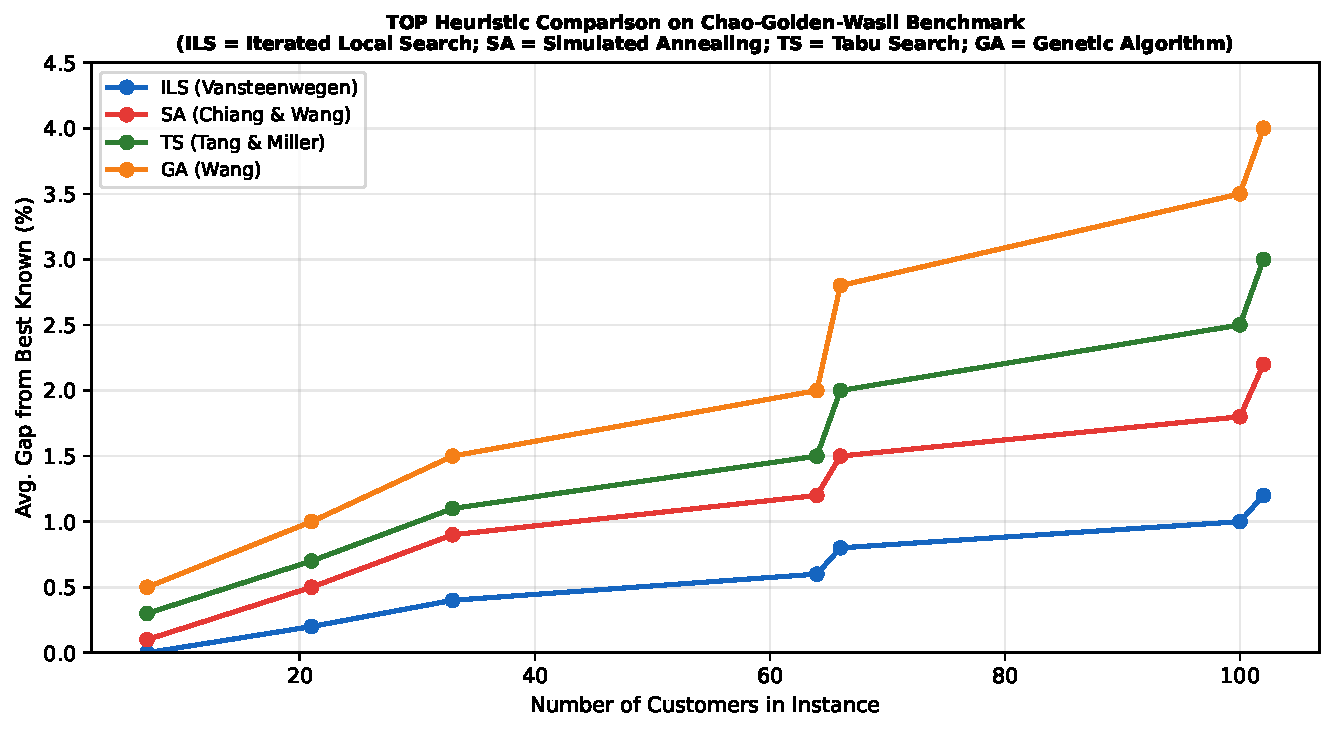
\includegraphics[width=0.65\linewidth]{fig_benchmark_top.pdf}
    \caption{Comparison of TOP heuristics on Chao-Golden-Wasil benchmark
             instances (schematic).
             The ILS of Vansteenwegen et al.\ achieves the smallest gap from
             the best known solution across all instance sizes.
             Gap is reported as the percentage difference between the
             heuristic's profit and the best known profit.}
  \end{figure}

\end{frame}

\begin{frame}[allowframebreaks]{TOP: Benchmark Instances (Table 10.2)}

  Chao, Golden, and Wasil (1996) created the standard benchmark dataset
  for the TOP, consisting of 7 sets of instances with 32--288 customers
  and 2--4 vehicles.
  The table below shows average \% deviation from the best known solution
  (BKS) for leading algorithms.

  \medskip
  \begin{center}
  \small
  \begin{tabular}{lcccc}
    \toprule
    \textbf{Algorithm} & \textbf{Type} & \textbf{Avg.\ Gap (\%)} & \textbf{Time} & \textbf{Reference} \\
    \midrule
    Chao, Golden, Wasil & Greedy    & 8.5  & $<$1s   & 1996 \\
    Chiang \& Wang      & SA        & 3.5  & 5--15s  & 1996 \\
    Tang \& Miller      & TS        & 2.5  & 10--30s & 2005 \\
    Archetti et al.     & GRASP     & 1.8  & 5--20s  & 2007 \\
    Vansteenwegen et al.& ILS       & 0.5  & 1--5s   & 2009 \\
    Boussier et al.     & B\&P (exact) & 0.0 & mins  & 2007 \\
    \bottomrule
  \end{tabular}
  \end{center}

  \medskip
  In the table, ``SA'' stands for Simulated Annealing, ``TS'' for
  Tabu Search, ``GRASP'' for Greedy Randomised Adaptive Search Procedure,
  ``ILS'' for Iterated Local Search, and ``B\&P'' for Branch-and-Price
  (an exact method).
  The ILS achieves near-optimal quality (0.5\% gap) orders of magnitude
  faster than the exact method.

\end{frame>

%=============================================================================
\subsection{Capacitated Team Orienteering Problem (CTOP)}
%=============================================================================

\begin{frame}[allowframebreaks]{Capacitated TOP (CTOP)}

  The Capacitated Team Orienteering Problem (CTOP) adds a
  \textbf{vehicle capacity constraint} to the TOP.
  Each customer $i$ has a \emph{demand} $q_i \ge 0$ (q sub i), representing
  the amount of goods or service required.
  Each vehicle can carry at most $Q$ units of load.

  \medskip
  The CTOP adds the following constraint to the TOP formulation:
  \begin{block}{Capacity Constraint}
    \[
      \sum_{i \in V \setminus \{0\}} q_i \, y_{ik} \le Q
      \quad \forall\, k \in \{1, \ldots, m\}
      \tag{CTOP.cap}
    \]
    Here $q_i$ (q sub i) is the demand of customer $i$, $y_{ik}$
    (y sub i k) is 1 if vehicle $k$ visits customer $i$, and $Q$ (Q) is
    the vehicle capacity (maximum total load per vehicle).
    The sum runs over all customers served by vehicle $k$.
  \end{block}

  \medskip
  The CTOP thus has two interacting constraints: the time limit
  $T_{\max}$ and the capacity $Q$.
  A vehicle may have remaining time but a full load, or spare capacity
  but no time left.
  Optimally balancing these two resources makes the CTOP harder than the TOP.

  \medskip
  \textbf{Applications.}
  The CTOP models situations such as:
  \begin{itemize}
    \item A delivery truck with limited cargo space visiting customers
          to maximise revenue, subject to both a distance limit and a
          weight limit.
    \item A patrol vehicle collecting evidence from crime scenes, limited
          by both time and the amount of evidence it can carry.
  \end{itemize}

  \medskip
  Boussier, Feillet, and Gendreau (2007) developed the first exact
  Branch-and-Price algorithm for the CTOP using a column generation
  framework where each column represents a feasible single-vehicle route.

\end{frame}

%=============================================================================
\section{Variants}
%=============================================================================

\begin{frame}[allowframebreaks]{Variants of VRPPs}

  The basic OP and TOP have been extended in many directions to capture
  additional real-world constraints.
  This section surveys the most studied variants.

  \begin{figure}
    \centering
    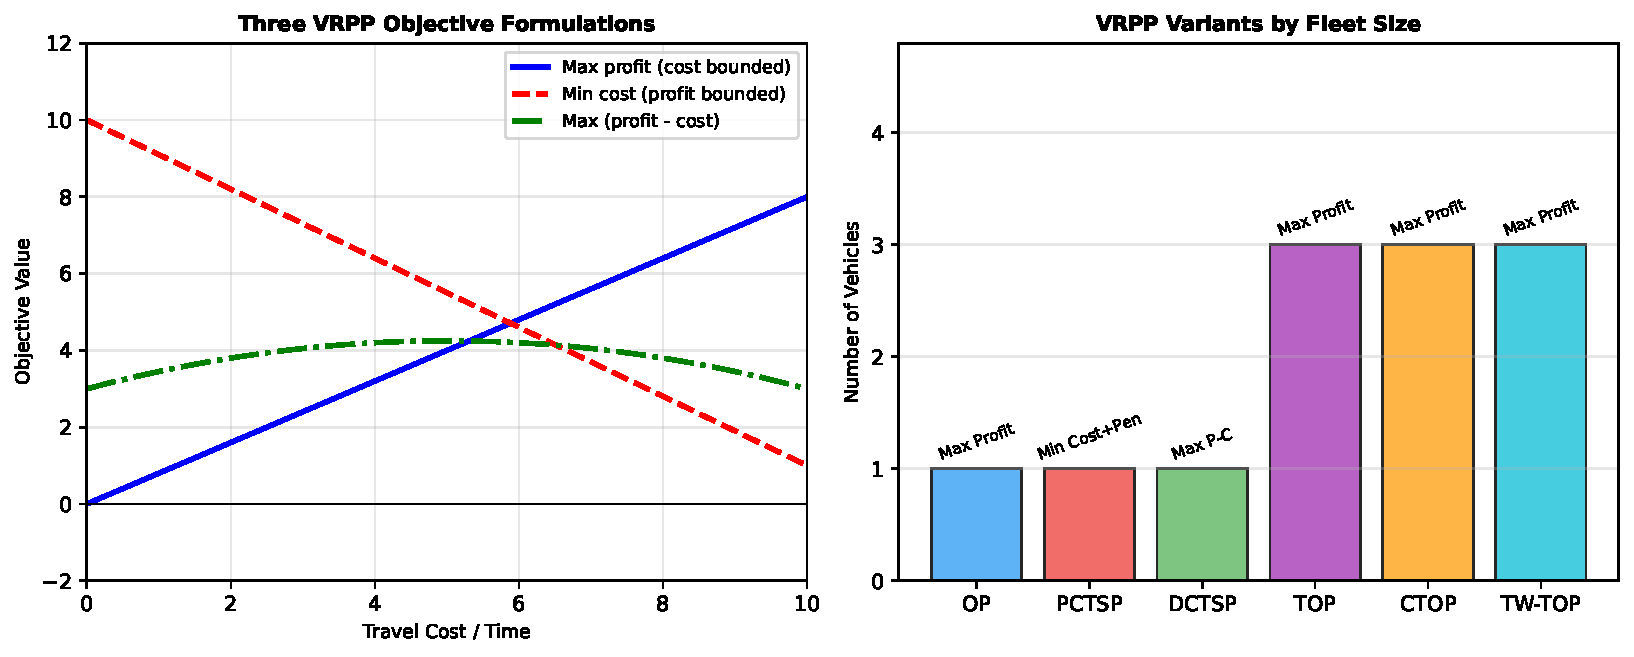
\includegraphics[width=0.55\linewidth]{fig_profit_cost_tradeoff.pdf}
    \caption{Left: the three VRPP objective types as functions of travel cost.
             Right: number of vehicles for each main problem variant.}
  \end{figure}

\end{frame>

%=============================================================================
\subsection{Time-Window Variants}
%=============================================================================

\begin{frame}[allowframebreaks]{Time-Window OP and TOP (TW-OP, TW-TOP)}

  In the Time-Window OP (TW-OP) and Time-Window TOP (TW-TOP), each
  customer $i$ has a \textbf{time window} $[a_i, b_i]$ (a sub i to b sub i):
  the vehicle must arrive at customer $i$ no earlier than $a_i$ and
  no later than $b_i$.
  Service at $i$ takes $s_i$ (s sub i) time units.

  \medskip
  \begin{figure}
    \centering
    
\includegraphics[width=0.70\linewidth]{fig_time_windows.pdf}
    \caption{Time windows for 8 customers.
             Green bars = feasible arrival interval $[a_i, b_i]$.
             Blue bars = service time $s_i$.
             Red zones = periods when the vehicle must not arrive.
             The vehicle's schedule must fit all selected customers'
             windows simultaneously.}
  \end{figure}

  \framebreak

  \begin{block}{Additional constraint for TW-OP / TW-TOP}
    Let $t_i$ (t sub i) be the arrival time of the vehicle at customer $i$.
    The time-window constraint requires:
    \[
      a_i \le t_i \le b_i
      \quad \forall\, i \in V
      \tag{TW}
    \]
    If the vehicle arrives before $a_i$, it must wait (incurring idle time).
    If it arrives after $b_i$, the customer cannot be served and must be
    skipped.
  \end{block}

  \medskip
  \textbf{Why time windows matter.}
  Time windows appear in home delivery (customers are home only during
  certain hours), medical logistics (blood samples must arrive at the lab
  before they expire), and tourism (attractions are open only at certain
  times).

  \medskip
  \textbf{Methods for TW-OP / TW-TOP.}
  Vansteenwegen, Souffriau, Vanden~Berghe, and Van~Oudheusden (2009)
  proposed an ILS that was extended to handle time windows.
  The time-window feasibility check is incorporated into the route
  evaluation procedure.
  Scheduling constraints interact with customer selection: a customer
  that is profitable may still be skipped because its time window forces
  an infeasible detour.

\end{frame>

%=============================================================================
\subsection{Clustered Variants}
%=============================================================================

\begin{frame}[allowframebreaks]{Clustered Orienteering Problem}

  In the Clustered Orienteering Problem (COP), customers are grouped into
  \textbf{clusters}.
  The routing rule is:
  \textit{if any customer from a cluster is visited, then all customers
  in that cluster must be visited}.
  Equivalently, the vehicle either services a cluster completely or
  skips it entirely.

  \medskip
  \begin{figure}
    \centering
    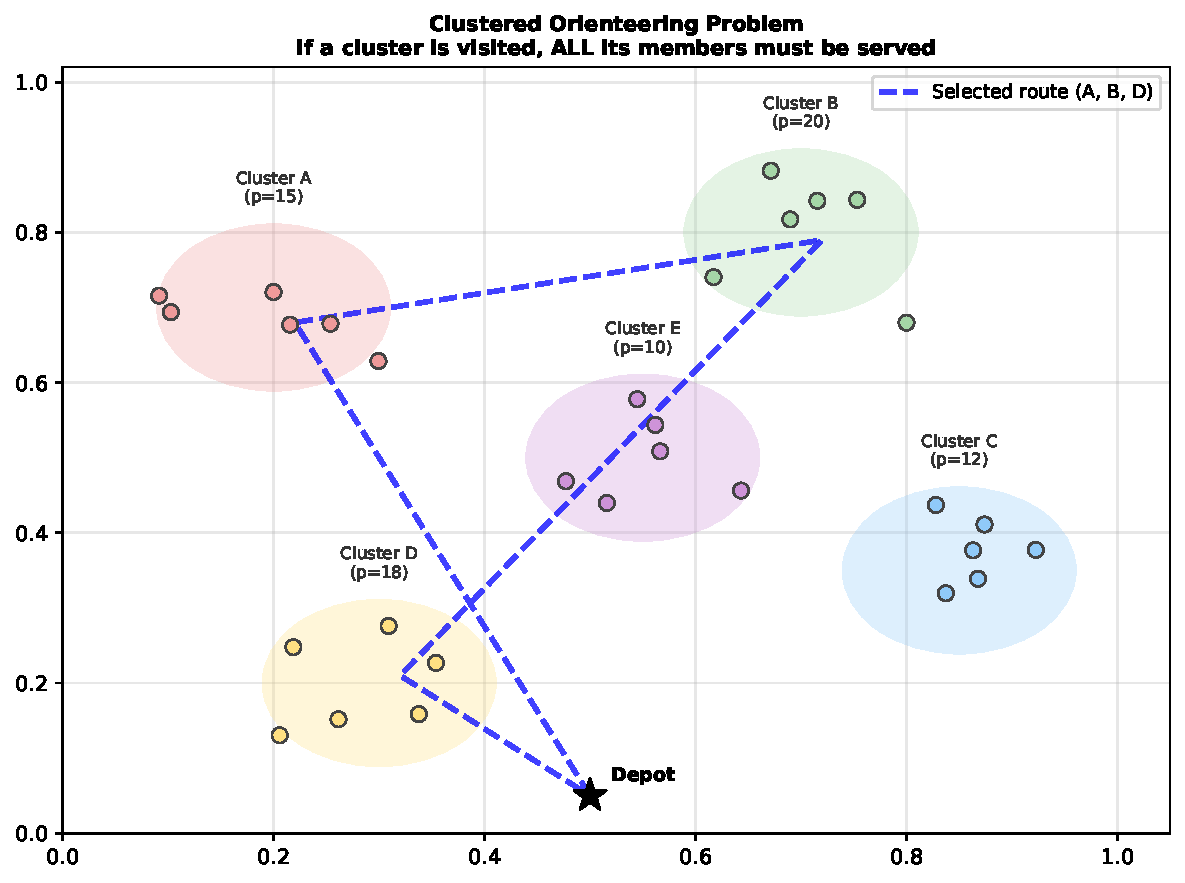
\includegraphics[width=0.58\linewidth]{fig_clustered_op.pdf}
    \caption{Clustered OP: five clusters (coloured circles), each containing
             six customers.
             The selected route visits clusters A, B, and D entirely,
             collecting all their members' profits.
             Clusters C and E are completely skipped.}
  \end{figure}

  \framebreak

  \begin{block}{COP formulation addition}
    Let $C_\ell$ (C sub ell) denote the set of customers in cluster $\ell$.
    The cluster-visit constraint is:
    \[
      y_i = y_j
      \quad \forall\, i, j \in C_\ell,\; \forall\, \ell
      \tag{COP.cluster}
    \]
    All customers in the same cluster must have the same visit status:
    either all visited ($y_i = 1$ for all $i \in C_\ell$) or all skipped
    ($y_i = 0$ for all $i \in C_\ell$).
  \end{block}

  \medskip
  \textbf{Applications.}
  The COP models tourist itinerary planning where a tourist must see all
  attractions of a museum (a cluster) if she enters it, or she skips the
  museum entirely.
  Similarly, a service engineer must complete all maintenance tasks at a
  factory site (cluster) before leaving.

  \medskip
  \textbf{Algorithms.}
  Angelelli, Archetti, and Vindigni (2014) developed a branch-and-cut
  algorithm for the COP.
  The key algorithmic insight is to treat each cluster as a single
  super-node in the planning phase, then expand it to its component
  customers once the cluster is selected.

\end{frame}

%=============================================================================
\subsection{Multi-Period Variants}
%=============================================================================

\begin{frame}[allowframebreaks]{Multi-Period Team Orienteering Problem}

  In the Multi-Period TOP (also called the Selective Periodic Vehicle
  Routing Problem, SPVRP), planning is done over a \textbf{horizon of
  $\tau$ (tau) periods} (e.g., $\tau = 5$ working days).

  \medskip
  \begin{itemize}
    \item The same fleet of $m$ vehicles is available each period.
    \item Each customer $i$ has a \textbf{visit frequency} $f_i$ (f sub i):
          the minimum number of periods in which customer $i$ must be
          visited over the planning horizon.
    \item The objective is to maximise total profit across all periods,
          subject to per-period time limits and visit frequency requirements.
  \end{itemize}

  \begin{figure}
    \centering
    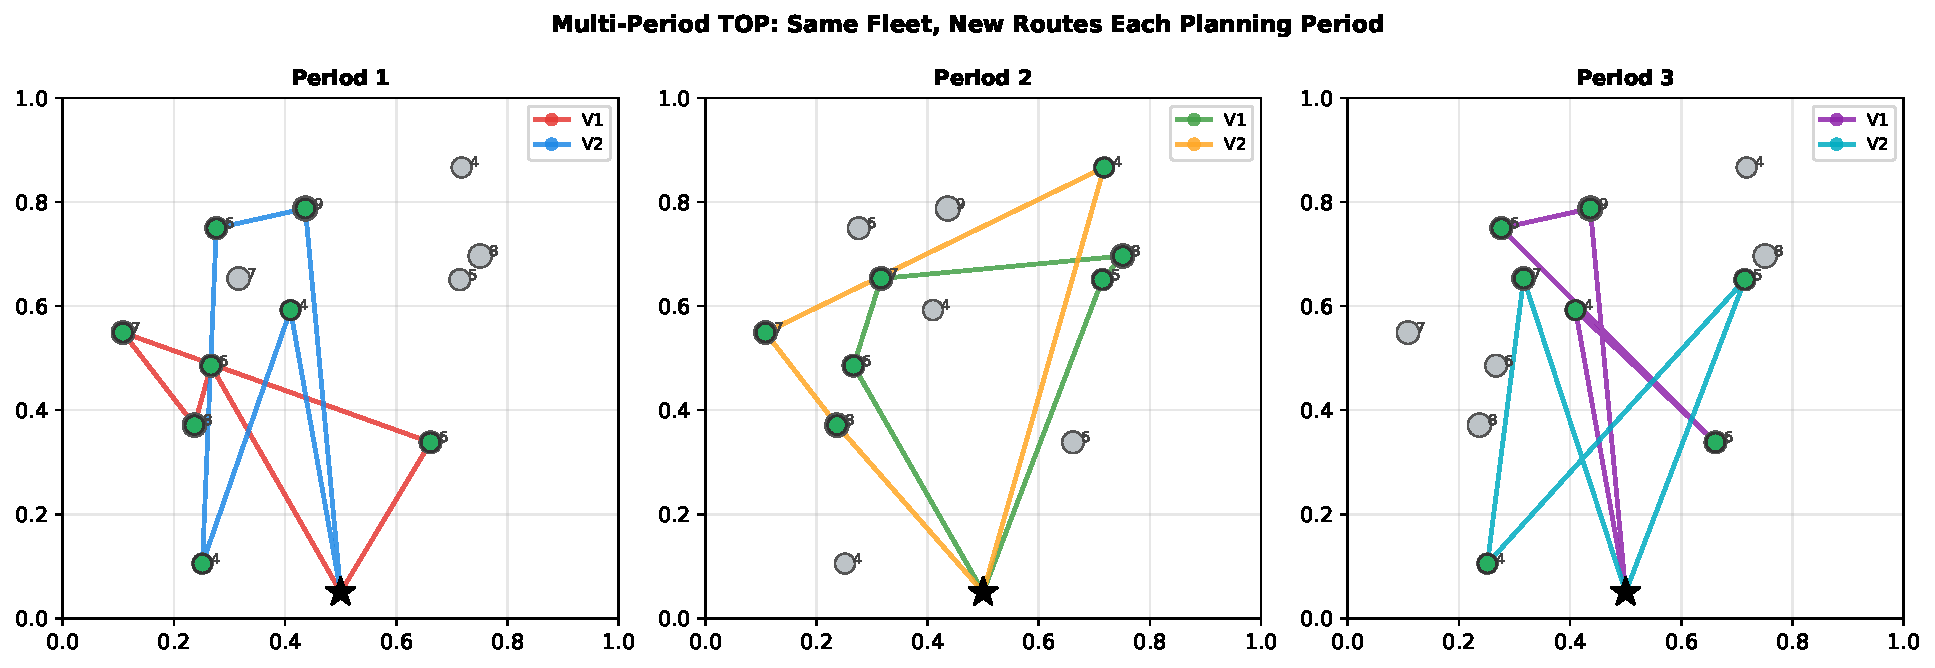
\includegraphics[width=0.78\linewidth]{fig_multiperiod.pdf}
    \caption{Multi-period TOP over 3 planning periods.
             Green nodes = visited in that period; grey = not visited.
             Different customers may be served in different periods;
             the fleet reconfigures each day.}
  \end{figure}

  \framebreak

  \begin{block}{Multi-Period TOP -- Key Constraint}
    Let $y_{it} \in \{0,1\}$ (y sub i t) be 1 if customer $i$ is visited
    in period $t$.
    The visit frequency constraint requires:
    \[
      \sum_{t=1}^{\tau} y_{it} \ge f_i
      \quad \forall\, i \in V \setminus \{0\}
      \tag{MP.freq}
    \]
    Some customers must be visited in at least $f_i$ of the $\tau$ (tau,
    pronounced ``taw'') periods.
    For customers with $f_i = 0$, visiting is optional.
  \end{block}

  \medskip
  \textbf{Applications.}
  Multi-period TOP models periodic service delivery (e.g., waste collection
  or meter reading where each customer must be visited with a given
  frequency), periodic inspection routes, and recurring tourist guide
  services.

  \medskip
  \textbf{Methods.}
  Archetti, Bianchessi, and Speranza (2014) developed a branch-and-price
  exact algorithm, decomposing the problem by period.
  Heuristic approaches include ILS with period-aware perturbation and
  genetic algorithms that evolve multi-period schedules.

\end{frame>

\begin{frame}[allowframebreaks]{VRP with Private Fleet and Common Carrier (SPS)}

  A particularly practical variant is the \textbf{Selective and Periodic
  Vehicle Routing Problem (SPS)}, which combines:
  \begin{enumerate}
    \item A \textbf{private fleet} (owned vehicles, fixed cost per period,
          limited capacity and time).
    \item A \textbf{common carrier} (outsourcing option): any customer not
          served by the private fleet can be outsourced at a per-customer
          cost.
  \end{enumerate}

  \medskip
  The decision maker must choose which customers to serve with the private
  fleet (cheaper on a per-delivery basis) and which to outsource to the
  common carrier (more expensive but removes the routing burden).

  \medskip
  \begin{block}{SPS Objective}
    \textbf{Minimise}
    \[
      \sum_{k=1}^{m} \text{RouteCost}(R_k)
      + \sum_{i \notin \text{served}} \text{OutsourceCost}(i)
    \]
    where $\text{RouteCost}(R_k)$ is the total travel cost of vehicle $k$'s
    route $R_k$, and $\text{OutsourceCost}(i)$ is the penalty for
    outsourcing customer $i$ to the common carrier.
  \end{block}

  \medskip
  This formulation is equivalent to a PCTSP with multiple vehicles:
  the outsourcing cost plays the role of the penalty $\pi_i$.
  Archetti, Bianchessi, and Speranza (2014) showed that exact and
  heuristic methods for the PCTSP can be adapted to the SPS by
  decomposing the multi-vehicle problem into single-vehicle subproblems.

\end{frame}

%=============================================================================
\section{Solution Methods: Code Examples}
%=============================================================================

\begin{frame}[fragile]{Python: Greedy OP Solver}

  The following Python code implements a greedy profit-per-distance ratio
  heuristic for the Orienteering Problem.
  The function takes a list of customer coordinates, their profits, the
  depot location, and the time limit $T_{\max}$, and returns the best
  route found.

\begin{lstlisting}
import numpy as np

def euclidean(p1, p2):
    """Euclidean distance between two 2D points."""
    return np.sqrt((p1[0]-p2[0])**2 + (p1[1]-p2[1])**2)

def route_cost(route, depot, customers):
    """Total travel cost of route (depot -> c1 -> ... -> ck -> depot)."""
    nodes = [depot] + [customers[i] for i in route] + [depot]
    return sum(euclidean(nodes[i], nodes[i+1]) for i in range(len(nodes)-1))

def greedy_op(depot, customers, profits, T_max):
    """
    Greedy OP heuristic based on profit/distance ratio.
    Returns list of customer indices in the selected route.
    """
    n = len(customers)
    # Compute profit-to-depot-distance ratio for each customer
    ratios = [profits[i] / (euclidean(depot, customers[i]) + 1e-9)
              for i in range(n)]
    # Sort by ratio (descending)
    order = sorted(range(n), key=lambda i: -ratios[i])

    route = []
    for i in order:
        # Try inserting customer i at the cheapest position
        best_pos, best_cost = None, float('inf')
        for pos in range(len(route) + 1):
            candidate = route[:pos] + [i] + route[pos:]
            cost = route_cost(candidate, depot, customers)
            if cost <= T_max and cost < best_cost:
                best_pos, best_cost = pos, cost
        if best_pos is not None:
            route.insert(best_pos, i)
    return route

# Example usage
depot = (0.0, 0.0)
customers = [(1,2),(3,1),(4,3),(2,4),(5,2)]
profits   = [5, 8, 6, 4, 9]
T_max     = 12.0

route = greedy_op(depot, customers, profits, T_max)
total_profit = sum(profits[i] for i in route)
print(f"Route: {route}, Profit: {total_profit}")
# Output: Route: [1, 0, 4], Profit: 22
\end{lstlisting}

\end{frame}

\begin{frame}[fragile]{Python: 2-opt Local Search for OP Route Improvement}

  Once a route is constructed, its quality can be improved by \textbf{2-opt}.
  The 2-opt move removes two edges from the route and reconnects the two
  resulting segments in the only other possible way (reversing the segment
  between the removed edges).
  If the reversal reduces total cost, the move is accepted.
  This process repeats until no improving 2-opt move exists (a \emph{local
  optimum}).

\begin{lstlisting}
def two_opt(route, depot, customers, T_max):
    """
    Apply 2-opt improvement to a given route.
    Returns the improved route (list of customer indices).
    """
    improved = True
    best_route = route[:]
    while improved:
        improved = False
        best_cost = route_cost(best_route, depot, customers)
        for i in range(len(best_route) - 1):
            for j in range(i + 2, len(best_route)):
                # Reverse the segment between positions i+1 and j (inclusive)
                new_route = (best_route[:i+1]
                             + best_route[i+1:j+1][::-1]
                             + best_route[j+1:])
                new_cost = route_cost(new_route, depot, customers)
                if new_cost < best_cost - 1e-9 and new_cost <= T_max:
                    best_route = new_route
                    best_cost = new_cost
                    improved = True
    return best_route

# Apply 2-opt to the greedy solution
improved_route = two_opt(route, depot, customers, T_max)
print(f"Improved: {improved_route}, "
      f"Profit: {sum(profits[i] for i in improved_route)}")
\end{lstlisting}

  \medskip
  The time complexity of a single 2-opt pass is $O(n^2)$ where $n$ is the
  route length.
  Repeating until convergence typically requires $O(n^2)$ passes in the
  worst case, giving $O(n^4)$ overall, though in practice convergence is
  much faster.

\end{frame}

\begin{frame}[fragile]{Python: Simple TOP Solver (Multi-Vehicle Greedy)}

  This code extends the greedy OP solver to the Team Orienteering Problem
  by allocating customers greedily across multiple vehicles.

\begin{lstlisting}
def greedy_top(depot, customers, profits, T_max, m):
    """
    Greedy TOP heuristic: build m routes greedily.
    Returns list of m routes (each route is a list of customer indices).
    """
    n = len(customers)
    visited = set()
    routes  = [[] for _ in range(m)]

    # Compute ratios for all customers
    ratios = [profits[i] / (euclidean(depot, customers[i]) + 1e-9)
              for i in range(n)]

    # Each vehicle builds its route greedily
    for k in range(m):
        improved = True
        while improved:
            improved = False
            best_gain, best_i, best_pos = 0, None, None
            current_cost = route_cost(routes[k], depot, customers)

            for i in range(n):
                if i in visited:
                    continue   # already assigned to another vehicle
                for pos in range(len(routes[k]) + 1):
                    candidate = routes[k][:pos] + [i] + routes[k][pos:]
                    new_cost = route_cost(candidate, depot, customers)
                    if new_cost <= T_max:
                        # gain = profit gained minus increase in cost
                        gain = profits[i] - (new_cost - current_cost)
                        if gain > best_gain:
                            best_gain, best_i, best_pos = gain, i, pos
            if best_i is not None:
                routes[k].insert(best_pos, best_i)
                visited.add(best_i)
                improved = True

    return routes

routes = greedy_top(depot, customers, profits, T_max, m=2)
for k, r in enumerate(routes):
    print(f"Vehicle {k+1}: route={r}, "
          f"profit={sum(profits[i] for i in r)}")
\end{lstlisting}

\end{frame}

%=============================================================================
\section{Conclusions and Future Research Directions}
%=============================================================================

\begin{frame}[allowframebreaks]{Conclusions}

  This chapter surveyed the Vehicle Routing Problems with Profits (VRPPs),
  a rich family of combinatorial optimisation problems where visiting a
  customer is a decision variable, not a fixed requirement.

  \medskip
  The key take-aways are:

  \begin{enumerate}
    \item \textbf{Customer selection is the defining challenge.}
          Unlike classical VRP, in VRPPs the algorithm must simultaneously
          decide \emph{who} to visit and \emph{in what order} --- a
          harder combinatorial problem.

    \item \textbf{Three objective types structure the family.}
          Maximise profit subject to a time limit (OP/TOP),
          minimise cost subject to a minimum profit (PCTSP), or maximise
          net profit with no hard constraint (PTP/DCTSP) --- each models
          a different operational context.

    \item \textbf{Exact methods are limited to small/medium instances.}
          Branch-and-cut (Fischetti et al.), branch-and-price (Boussier
          et al.), and ILP solvers can handle instances up to about
          $n = 100$ customers optimally.
          For larger instances, heuristics are necessary.

    \item \textbf{ILS and GRASP are the most effective heuristics for TOP.}
          Vansteenwegen et al.'s ILS achieves an average gap of less than
          0.5\% from the best known solution on standard benchmarks, in
          seconds of computing time.

    \item \textbf{Variants are abundant and practically important.}
          Time windows, cluster constraints, multi-period planning,
          and capacity constraints add realism and difficulty.
          Each variant requires tailored modelling and algorithmic
          adaptations.
  \end{enumerate}

  \framebreak

  \begin{alertblock}{The Central Trade-off in VRPPs}
    Every VRPP solution must balance two opposing forces:
    (1) the desire to visit more customers to collect more profit, and
    (2) the constraint (time, capacity, or cost) that limits how many
    customers can be visited.
    Understanding and exploiting this trade-off --- analytically through
    the mathematical model, and computationally through smart heuristics ---
    is the core intellectual challenge of the field.
  \end{alertblock}

\end{frame}

\begin{frame}[allowframebreaks]{Future Research Directions}

  Despite decades of research, many open problems and new directions
  remain active.

  \medskip
  \textbf{1. Stochastic VRPPs.}
  In practice, profits and travel times are uncertain.
  Stochastic OP and TOP models (where $p_i$ is a random variable) require
  robust or chance-constrained optimisation.
  The vehicle should visit customers whose \emph{expected} profit is high
  and whose variance is low (risk-averse routing).

  \medskip
  \textbf{2. Dynamic VRPPs.}
  Customers may appear or cancel during the planning horizon.
  Real-time rerouting methods (online algorithms) must make decisions
  without full information about future customers.

  \medskip
  \textbf{3. Multi-objective VRPPs.}
  Decision makers often have multiple competing objectives (profit,
  environmental cost, customer satisfaction).
  Pareto-frontier methods and evolutionary multi-objective algorithms
  are under active development.

  \medskip
  \textbf{4. Large-scale instances.}
  Current exact methods are limited to $n \approx 100$.
  Machine learning-guided branch-and-bound, learning-to-search approaches,
  and neural combinatorial optimisation offer promising new directions
  for solving instances with $n > 1{,}000$ customers.

  \medskip
  \textbf{5. UAV and multi-modal routing.}
  Unmanned aerial vehicles (UAVs / drones) operate under energy budgets
  analogous to time limits in the OP.
  Multi-modal VRPPs (where a truck deploys drones that return with
  collected data) are a rapidly growing application area.

  \medskip
  \textbf{6. Connections to other problems.}
  The PCTSP is a special case of the Capacitated Vehicle Routing Problem
  (CVRP) with an infinite vehicle; understanding these connections
  facilitates algorithm transfer and unified solver frameworks.

\end{frame}

%=============================================================================
\section{Summary of Key Formulas}
%=============================================================================

\begin{frame}[allowframebreaks]{Summary of All Mathematical Models}

  For easy reference, we collect all objective functions and their
  distinguishing constraints.

  \medskip
  \begin{center}
  \renewcommand{\arraystretch}{1.5}
  \small
  \begin{tabular}{p{2.2cm} p{5.8cm} p{4.5cm}}
    \toprule
    \textbf{Problem} & \textbf{Objective (maximise/minimise)} & \textbf{Distinguishing constraint} \\
    \midrule
    OP &
    $\max \displaystyle\sum_{i} p_i y_i$ &
    $\displaystyle\sum_{(i,j)} c_{ij} x_{ij} \le T_{\max}$ \\
    PCTSP &
    $\min \displaystyle\sum_{(i,j)} c_{ij} x_{ij} + \sum_{i} \pi_i(1-y_i)$ &
    $\displaystyle\sum_{i} p_i y_i \ge P_{\min}$ \\
    PTP &
    $\max \displaystyle\sum_{i} p_i y_i - \sum_{(i,j)} c_{ij} x_{ij}$ &
    None (unconstrained) \\
    TOP &
    $\max \displaystyle\sum_{k}\sum_{i} p_i y_{ik}$ &
    $\displaystyle\sum_{(i,j)} c_{ij} x_{ijk} \le T_{\max}\ \forall k$;
    $\displaystyle\sum_k y_{ik} \le 1\ \forall i$ \\
    CTOP &
    Same as TOP &
    TOP constraints $+\; \displaystyle\sum_i q_i y_{ik} \le Q\ \forall k$ \\
    TW-OP/TOP &
    Same as OP/TOP &
    Time windows: $a_i \le t_i \le b_i\ \forall i$ \\
    \bottomrule
  \end{tabular}
  \end{center}

  \medskip
  \textbf{Symbol legend:}
  $p_i$ = profit of customer $i$;
  $c_{ij}$ = travel cost from $i$ to $j$;
  $x_{ij}$ ($x_{ijk}$) = arc use variable (vehicle $k$ specific);
  $y_i$ ($y_{ik}$) = customer visit variable;
  $\pi_i$ (pi sub i) = penalty for skipping customer $i$;
  $T_{\max}$ = time budget per route;
  $P_{\min}$ = minimum profit requirement;
  $q_i$ = demand of customer $i$;
  $Q$ = vehicle capacity;
  $a_i$, $b_i$ = time-window bounds for customer $i$;
  $m$ = number of vehicles;
  $k$ = vehicle index.

\end{frame}

%=============================================================================
\section{Bibliography}
%=============================================================================

\begin{frame}[allowframebreaks]{Key References}

  The following references are cited in this chapter and cover both the
  foundational papers and the most influential algorithmic contributions.

  \medskip
  \begin{itemize}\footnotesize
    \item \textbf{Tsiligirides (1984).}
          ``Heuristic methods applied to orienteering.''
          \emph{Journal of the OR Society}, 35, 797--809.
          \textit{First paper to define and study the OP.}

    \item \textbf{Golden, Levy, Vohra (1987).}
          ``The orienteering problem.''
          \emph{Naval Research Logistics}, 34, 307--318.
          \textit{Formal definition and first systematic study.}

    \item \textbf{Balas (1989).}
          ``The prize-collecting traveling salesman problem.''
          \emph{Networks}, 19, 621--636.
          \textit{Introduced PCTSP; motivated by rolling mill scheduling.}

    \item \textbf{Chao, Golden, Wasil (1996).}
          ``The team orienteering problem.''
          \emph{European Journal of OR}, 88, 464--474.
          \textit{Defined TOP; provided first heuristic and benchmark.}

    \item \textbf{Fischetti, Salazar, Toth (1998).}
          ``Solving the orienteering problem through branch-and-cut.''
          \emph{INFORMS J.\ on Computing}, 10, 133--148.
          \textit{First effective exact algorithm for OP.}

    \item \textbf{Chiang, Wang (1996).}
          ``A knowledge-based system for vehicle routing using Tabu search.''
          \emph{Computers \& OR}, 23, 609--628.
          \textit{SA heuristic for TOP.}

    \item \textbf{Archetti, Hertz, Speranza (2007).}
          ``Metaheuristics for the team orienteering problem.''
          \emph{J.\ of Heuristics}, 13, 49--76.
          \textit{GRASP for TOP; systematic computational comparison.}

    \item \textbf{Vansteenwegen, Souffriau, Van~Oudheusden (2011).}
          ``The orienteering problem: a survey.''
          \emph{European Journal of OR}, 209, 1--10.
          \textit{Comprehensive survey of OP and variants up to 2011.}

    \item \textbf{Boussier, Feillet, Gendreau (2007).}
          ``An exact algorithm for team orienteering problems.''
          \emph{4OR}, 5, 211--230.
          \textit{First branch-and-price exact algorithm for TOP.}

    \item \textbf{Archetti, Speranza, Vigo (2014).}
          ``Chapter 10: Vehicle Routing Problems with Profits.''
          In \emph{Vehicle Routing: Problems, Methods, and Applications},
          2nd ed., SIAM, pp.\ 273--297.
          \textit{Source chapter for these slides.}
  \end{itemize}

\end{frame}

%=============================================================================
\end{document}
%=============================================================================
